\chapter{Diskuze} % Vysvětluje, co výsledky znamenají
\label{ch:diskuze}
% Interpretace výsledků = co znamenají.
% Porovnání s literaturou: odpovídají výsledky očekáváním? V čem se liší?
% Vysvětlení možných příčin, omezení, nejistot, překvapení.
% Reflexe metod: byly vhodně zvoleny? Co by šlo udělat lépe?
% Možné dopady, návrhy pro budoucí výzkum.

% - „Tento výsledek může být způsoben tím, že…“,
% - „Na rozdíl od práce XY jsme zaznamenali…“,
% - „Překvapivě model selhal při…“
Tato kapitola se věnuje interpretaci dosažených výsledků při odhadu srdeční tepové frekvence (\acs{TF}) ze signálu \acs{PPG} pomocí tří odlišných metod: Elgendiho algoritmu, vlastního algoritmu detekce vrcholů a přístupu založeného na Hjorthových deskriptorech.
Uvedené metody byly testovány na dvou databázích: CapnoBase a BUT PPG.

Samostatně je diskutováno také automatické hodnocení kvality signálu na základě Shannonovy entropie a indexu spektrální čistoty (\acs{SPI}).

%%%%%%%%%%%%%%%%%%%%%%%%%%%%%%%%%%%%%%%%%%%%%%%%%%%%%
%                     CapnoBase                     %
%%%%%%%%%%%%%%%%%%%%%%%%%%%%%%%%%%%%%%%%%%%%%%%%%%%%%
\section[Interpretace výkonu metod odhadu TF pro CapnoBase]{Interpretace výkonu metod odhadu TF pro\\CapnoBase}
% Cíl: Zdůraznit, co jsem zjistil a proč je to důležité.
% KEEP IN MIND: co výsledek „znamená“, nejen „je vysoký Se“
Na databázi CapnoBase dosahují obě metody detekce vrcholů (Elgendi a vlastní algoritmus) vysoké hodnoty \acs{Se} i \acs{PPV}, což se projevuje velmi nízkou průměrnou absolutní chybou (\acs{MAE} $\approx$ 0,34~\acs{bpm}).
Srovnání metod na Obr.~\ref{fig:capnobase_SePPV_1min} a Obr.~\ref{fig:capnobase_SePPV_8min} ukazuje, že vlastní algoritmus vykazuje mírně nižších hodnot \acs{Se}, tedy detekuje méně skutečných vrcholů, avšak zároveň dosahuje o něco vyšší hodnoty \acs{PPV}, což naznačuje nižší podíl falešně pozitivních detekcí.

Nejnižší hodnota \acs{Se} pro vlastní detekci byla zaznamenána ve druhé minutě signálu 0115, kde silná respirační složka výrazně ovlivnila rozsah systolické vlny (viz Obr.~\ref{fig:capnobase_our_err}).
Prahová hodnota, kterou jsme při kontrukci algoritmu zvolili, nebyla adaptabilní a v tomto případě byla nastavena na příliš vysokou hodnotu, takže náš algoritmus detekoval méně vrcholů, než bylo žádoucí.
Možnost opravy by bylo zvýšit spodní mezní frekvenci použitého filtru, čímž bychom utlumili respirační složku signálu.

Naproti tomu u signálu 0312 (Obr.~\ref{fig:our_elgendi_comparison}) dosáhl náš algoritmus vyššího \acs{PPV} díky konzervativnějšímu nastavení prahu, které umožnilo vyloučení falešných maxim.

\begin{figure}[ht]
	\centering
	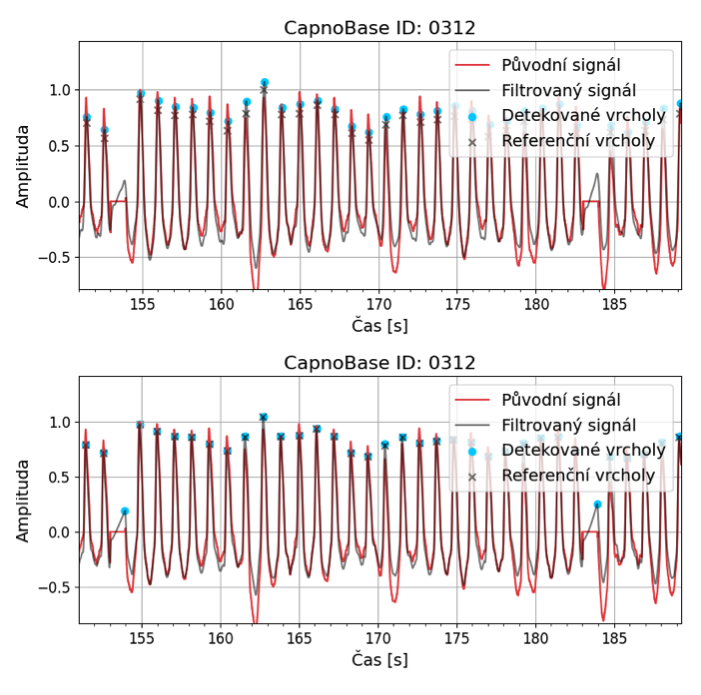
\includegraphics[width=1\textwidth]{./obrazky/diskuze/PPV_our_elgendi.png}
	\caption[Porovnání výkonu metod detekce vrcholů - CapnoBase]{Porovnání výkonu metod detekce vrcholů - CapnoBase.}
	\label{fig:our_elgendi_comparison}
\end{figure}

Vzhledem k velmi podobnému skóre \acs{F1} lze obě detekční metody považovat za srovnatelně výkonné.
U všech signálů (osmiminutových i minutových) splňují požadavek mezinárodní normy IEC~60601-2-27, která stanovuje maximální odchylku od referenční \acs{TF} $\pm$5~\acs{bpm}.

Metoda založená na Hjorthových deskriptorech vykazuje pro celou délku signálů vyšší průměrnou chybu (\acs{MAE} = 1,52~\acs{bpm}), její výkonnost se však výrazně zlepšuje s kratšími segmenty.
Při analýze desetisekundových úseků dosahuje průměrné chyby pouze 0,61~\acs{bpm}, což je velmi slibný výsledek.
Oproti metodám detekce vrcholů, jejichž přesnost je víceméně konstantní, je zde patrná závislost na délce segmentu, což by v praktických aplikacích vyžadovalo optimalizaci délky vstupního signálu.

Vedle \acs{MAE} byla hodnocena i úspěšnost metody z hlediska podílu segmentů, které splňují požadavky normy IEC.
Výsledky jsou v tomto ohledu horší než u detekčních algoritmů, nicméně pro krátké a kvalitní segmenty dosahuje Hjorthova metoda velmi dobrých výsledků.
Zejména u desetisekundových segmentů byla identifikována pouze jediná instance nesplňující kritérium odchylky, přičemž šlo o signál výrazně zatížený artefakty a vyhodnocený jako nekvalitní na základě metriky O-SQI (viz Obr.~\ref{fig:capnobase_hjorth_err}).

Lze tedy konstatovat, že pro krátké, kvalitní segmenty signálů z databáze CapnoBase dosahuje metoda založená na Hjorthových parametrech 100\% úspěšnosti v rámci požadavků IEC~60601-2-27.

Pro posouzení systematických odchylek mezi odhadem a referencí byla provedena Bland-Altmanova analýza (Obr.~\ref{fig:capnobase_BlandAltman_peaks} a Obr.~\ref{fig:capnobase_BlandAltman_hjorth}).
U obou detekčních metod je patrná slabá závislost chyby na velikosti průměrné \acs{TF} (s rostoucí \acs{TF} narůstá rozptyl i výskyt extrémních chybových hodnot).
U Hjorthovy metody jsou hranice shod širší, a tedy i variabilita odhadu vyšší, nicméně průměrná chyba je srovnatelná.
Tato metoda navíc nevykazuje výraznou závislost na velikosti \acs{TF}, což by mohlo být výhodné při odhadu v dynamicky proměnných podmínkách.

Použití Hjorthovy mobility pro odhad \acs{TF} představuje inovativní přístup, který se ukázal jako slibný zejména v případě krátkých a kvalitních úseků signálu.

%%%%%%%%%%%%%%%%%%%%%%%%%%%%%%%%%%%%%%%%%%%%%%%%%%%%%
%                      BUT PPG                      %
%%%%%%%%%%%%%%%%%%%%%%%%%%%%%%%%%%%%%%%%%%%%%%%%%%%%%
\section[Interpretace výkonu metod odhadu TF pro BUT PPG]{Interpretace výkonu metod odhadu TF pro\\BUT PPG}
Vzhledem k absenci referenčních anotací systolických vrcholů v databázi BUT PPG bylo hodnocení výkonu metod omezeno na metriky založené na odhadu srdeční tepové frekvence (\acs{TF}).
Konkrétně byla použita průměrná absolutní chyba (\acs{MAE}), přičemž za přijatelnou byla považována hodnota menší než 5~\acs{bpm} v souladu s normou IEC~60601-2-27.

\begin{figure}[!ht]
	\centering
	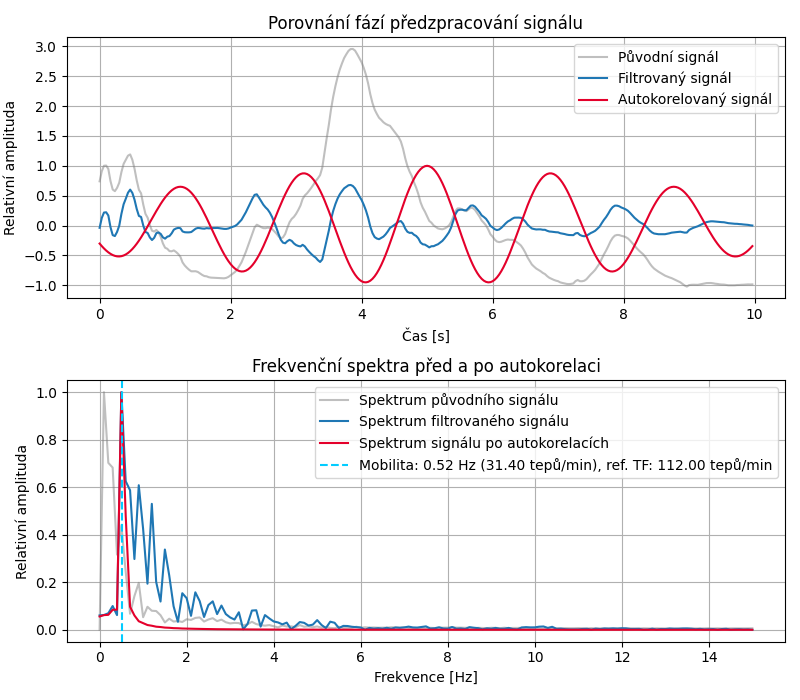
\includegraphics[width=1\textwidth]{./obrazky/diskuze/err_hjorth_but_1.png}
	\caption[Největší odchylky u Hjorthovy metody 1 - BUT PPG]{Největší odchylky u Hjorthovy metody 1.}
	\label{fig:BUT_hjorth_err_1}
\end{figure}

\begin{figure}[!ht]
	\centering
	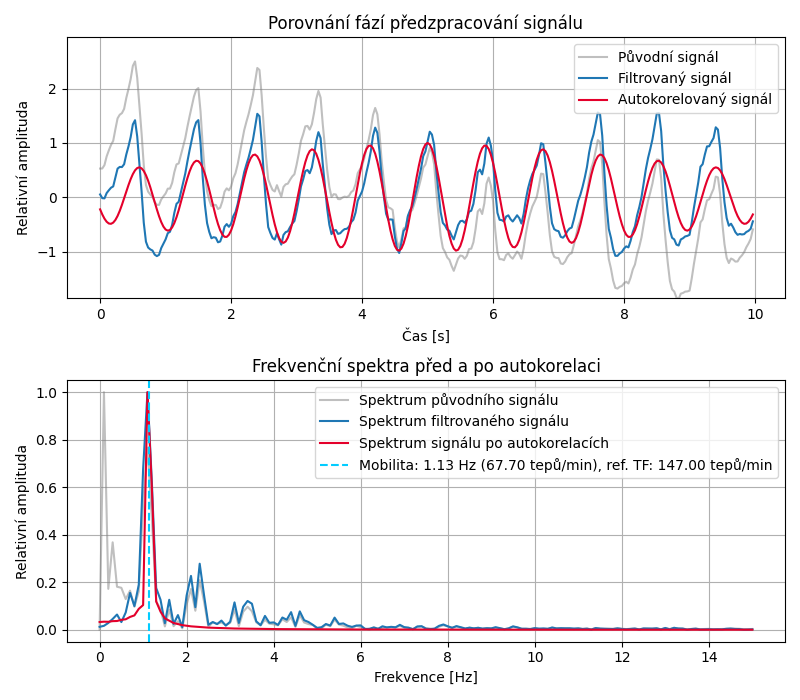
\includegraphics[width=1\textwidth]{./obrazky/diskuze/err_hjorth_but_2.png}
	\caption[Největší odchylky u Hjorthovy metody 2 - BUT PPG]{Největší odchylky u Hjorthovy metody 2.}
	\label{fig:BUT_hjorth_err_2}
\end{figure}

Jak ukazuje Tab.~\ref{tab:but_ppg_comparison}, všechny tři hodnocené metody vykazují na této databázi nižší přesnost než na CapnoBase, což lze přičíst přítomnosti většího množství signálů nízké kvality.
Elgendiho algoritmus dosahuje \acs{MAE} 18,84~\acs{bpm}, vlastní metoda 20,54~\acs{bpm} a metoda využívající Hjorthovy deskriptory 31,22~\acs{bpm}.

Po separaci kvalitních signálů pomocí referenčního skóre \acs{R-SQI} a skóre \acs{O-SQI} došlo u všech metod k výraznému zlepšení přesnosti.
Zatímco výkonnost detekčních metod se mezi oběma kritérii kvality příliš neliší, u Hjorthovy metody je zlepšení po aplikaci \acs{O-SQI} výraznější než po aplikaci \acs{R-SQI}.
Tato skutečnost naznačuje, že detekční algoritmy jsou obecně odolnější vůči zhoršené kvalitě signálu, zatímco metoda využívající Hjorthovu mobilitu je na kvalitu vstupu výrazně citlivější.

Bland-Altmanovy grafy (Obr.~\ref{fig:BUT_BlandAltman_elgendi} až \ref{fig:BUT_BlandAltman_hjorth}) dále ukazují, že selekce kvalitních signálů výrazně redukuje rozptyl rozdílů mezi odhadovanou a referenční \acs{TF}, přičemž největší variabilita se projevuje u Hjorthovy metody na celé databázi.
Zde se vyskytují i extrémní chybové hodnoty, zejména u signálů s vyšší průměrnou \acs{TF}, které metoda systematicky podhodnocuje (ME < 0).
V ojedinělých případech však dochází k opačnému efektu, kdy metoda významně přestřeluje, což vede k extrémně vysokým chybám.
Tato odlehlá pozorování jsou vizualizována v horní části grafu na Obr.~\ref{fig:BUT_BlandAltman_hjorth}.

Graf na Obr.~\ref{fig:BUT_hr_dif_O-SQI} dokumentuje chování Hjorthovy metody na podmnožině signálů označených jako kvalitní dle \acs{O-SQI}.
Horní panel ukazuje, že metoda má obecně tendenci \acs{TF} podhodnocovat, zatímco dolní panel ukazuje, že většina odhadů se pohybuje v přijatelném rozmezí, a pouze menší část vykazuje výraznou odchylku.
Výsledná průměrná absolutní chyba 8,05~\acs{bpm} je tedy tvořena několika odlehlými signály s velmi vysokou chybou, přesahující 60~\acs{bpm}, jak ilustrují Obr.~\ref{fig:BUT_hjorth_err_1} a Obr.~\ref{fig:BUT_hjorth_err_2}.

Souhrnně lze říci, že metoda založená na Hjorthově mobilitě vykazuje na kvalitních segmentech (dle \acs{O-SQI}) srovnatelný výkon s algoritmy detekce vrcholů.
Bez předchozí selekce kvality však její výstupy vykazují vysoký rozptyl a systematickou chybu, což výrazně omezuje její využitelnost v praxi.
Detekční algoritmy vykazují vyšší robustnost vůči artefaktům, přičemž Elgendiho algoritmus mírně překonává vlastní přístup z hlediska konzistence odhadu.

%%%%%%%%%%%%%%%%%%%%%%%%%%%%%%%%%%%%%%%%%%%%%%%%%%%%%
%                      Rychlost                     %
%%%%%%%%%%%%%%%%%%%%%%%%%%%%%%%%%%%%%%%%%%%%%%%%%%%%%
\section{Výpočetní náročnost metod odhadu TF}
Z hlediska výpočetní náročnosti byly všechny testované metody dostatečně rychlé pro potenciální nasazení v reálném čase.
Nejrychlejší z nich byl Elgendiho algoritmus.
V případě implementace v knihovně \texttt{NeuroKit2} bylo však nutné deaktivovat defaultní výpočet kvality signálu, neboť ten výrazně prodlužoval celkový čas zpracování.

Vlastní metoda detekce vrcholů a Hjorthova metoda byla mírně pomalejší, ale stále plně použitelná v praxi.

Větší rozdíly se daly vypozorovat na \acs{BUT PPG} databázi.
O pár sekund nejrychlejší byl vlastní algoritmus detekce vrcholů, následovaný Elgendiho algoritmem.
Hjorthova metoda byla nejpomalejší, což může být způsobenou vyšší asymptotickou složitostí výpočtu.

%%%%%%%%%%%%%%%%%%%%%%%%%%%%%%%%%%%%%%%%%%%%%%%%%%%%%
%                      Kvalita                      %
%%%%%%%%%%%%%%%%%%%%%%%%%%%%%%%%%%%%%%%%%%%%%%%%%%%%%
\section[Hodnocení automatického stanovení kvality signálů]{Hodnocení automatického stanovení kvality\\signálů}
Pro automatické hodnocení kvality \acs{PPG} signálů byl použit klasifikátor náhodného lesa trénovaný na dvojici příznaků: Shannonově entropii a spektrálním indexu výkonu (\acs{SPI}).
Na sloučené databázi CapnoBase a BUT PPG dosáhl model vysoké klasifikační schopnosti s hodnotou plochy pod ROC křivkou (\acs{AUC}) rovnou $0,957$ (viz Obr.~\ref{fig:roc_kvalita}).
ROC křivka ukazuje výraznou separaci mezi třídami, přičemž vyšší hodnoty \acs{SPI} a nižší Shannonova entropie korelují s vyšší kvalitou signálu, což potvrzuje informační přínos obou příznaků.

Ve scatterplotu (Obr.~\ref{fig:scatterplot_kvalita}) je patrná tendence k oddělení tříd, avšak bez jednoznačně definované rozhodovací hranice.
Nejvyšší klasifikační přesnosti bylo dosaženo při tréninku na kombinované databázi, zatímco výkon na jednotlivých databázích odděleně byl výrazně nižší.
Zhoršení výkonu pravděpodobně souvisí s výraznou nevyvážeností tříd a rozdílným poměrem kvalitních a nekvalitních signálů mezi oběma databázemi.

Zejména na databázi BUT PPG vykazoval klasifikátor sníženou schopnost identifikovat kvalitní signály, což lze přičíst větší variabilitě dat, přítomnosti artefaktů odlišného charakteru a rozdílné morfologii signálů.
Výsledky tedy ukazují, že i přes vysoký výkon na spojené databázi není možné s dostatečnou jistotou tvrdit, že model bude spolehlivě fungovat na dosud neznámých datech.
Je možné, že model se částečně naučil rozlišovat mezi konkrétními databázemi, nikoli mezi kvalitou signálu jako takovou.

Zvýšení klasifikační výkonnosti by mohlo být dosaženo jednak rozšířením množiny vstupních příznaků (například o další spektrální, morfologické či nelineární charakteristiky), jednak použitím rozsáhlejších, vyváženějších a více heterogenních trénovacích dat, která by reprezentovala širší spektrum typů \acs{PPG} signálů.